\documentclass[10pt,a4paper]{article}
\usepackage[utf8]{inputenc}
\usepackage{amsmath}
\usepackage{amsfonts}
\usepackage{amssymb}
\usepackage{graphicx}
\begin{document}
\section*{Security Analysis}
\subsection*{System Model}
\subsubsection*{Primitives}
Before defining the system model, all the cryptographic primitives used and their corresponding notations in this protocol should be described:
\begin{itemize}
\item Message Authentication Code $\mathcal{MAC}$\\
The MAC function used in this protocol is assumed to be secure in the sense that it has all the properties that a cryptographic hash function possesses and additionally, it resists to existential forgery under chosen-plaintext attack. That is, even if attacker is able to access an oracle which possesses the secret key and generates MACs according to the attacker's input, it is computational infeasible for attacker to guess MACs of other messages (not used to query the oracle).

\item Signature Function $\mathcal{SIGN}$\\
The signature function used in this protocol is assumed to be secure in the sense that it resists existential forgery under an adaptive chosen message attack. \cite{goldwasser}

\item Encryption Function $\mathcal{E}$ and Decryption Function $\mathcal{D}$\\
The notation $\mathcal{E}_k$ denotes an abstraction of all encryption functions, including both symmetric and asymmetric encryptions. Similarly, $\mathcal{D}_k$ represents both symmetric and asymmetric decryption functions. The subscript k denotes the key used for encryption/decryption processes.\\
To assure the security primitives of this protocol, all encryption/decryption schemes used are required to be secure in the sense that without the decryption key, it is computational infeasible for attackers to reveal the plaintext of a cipher with non-negligible probability.

\item Symmetric Key Generator $\mathcal{G}$\\
The symmetric key generator used in this protocol is assumed to be no less secure than a Cryptographically Secure Pseudorandom Number Generator. That is: \\
(a)It should satisfy the next-bit test. That is, given the first k bits of a random sequence, there is no polynomial-time algorithm that can predict the (k+1)th bit with probability of success better than 50\%. \\
(b)It should withstand "state compromise extensions". In the event that part or all of its state has been revealed (or guessed correctly), it should be impossible to reconstruct the stream of random numbers prior to the revelation. Additionally, if there is an entropy input while running, it should be infeasible to use knowledge of the input's state to predict future conditions of the CSPRNG state.\\
Furthermore, the keys generated are required to fit the Symmetric Encryption Scheme described above.
\\
(cite: from wikipedia)

\end{itemize}

\subsubsection*{Trusted entity model}
Totally 3 different types of entities are defined in the protocol:
\begin{itemize}
\item Alice $\mathcal{A}$, who creates the message and requests it to be delivered. It possesses an unique $\mathcal{ID} \in \{0, 1\}^*$, a secret key $sk_A$ as part of its asymmetric key pair, and the message $\mathcal{M}$ to be sent.
\item Bob $\mathcal{B}$, who is the recipient of the message. It possesses a unique secret key sk$_B$ as part of the asymmetric key pair. It possesses an unique $\mathcal{ID} \in \{0, 1\}^*$, and a secret key $sk_B$ as part of its asymmetric key pair.
\item Courier $\mathcal{C}$, who carries the message of Alice, physically transport from Alice to Bob, and delivers the message to Bob. Initially it only possesses an unique $\mathcal{ID} \in \{0, 1\}^*$ and a contact $\mathcal{ID} \in \{0, 1\}^*$ specifies the entity it is going to contact.\\
Specifically, a single Courier will play two different roles in the protocol run - one receives message from Alice, one delivers message to Bob. They are denoted as $\mathcal{CR}$ (Courier Receiver) and $\mathcal{CS}$ (Courier Sender). In addition, $\mathcal{CS}$ possesses some more information: the $\mathcal{ID}$ of the message creator, the encrypted message $\mathcal{E(M)} $ received from creator.
\end{itemize}

All trusted entities act as oracles $\prod_S$ who possess their own information (described above), take $\mathcal{M}$ as input, and output $\mathcal{M'}$. The $\mathcal{S}$ denotes its set of internal states which defines how $\prod$ responds to a certain input $\mathcal{M}$. (May add a figure of state machine) Its behaviour follows following procedure:
\begin{enumerate}
\item If $\prod \in \mathcal{C}$, initiate the protocol by sending ${\mathcal{M}_0}'$
\item Receive $\mathcal{M}_1$ and decrypt all its ciphertexts if applicable.
\item Check validity of the contents of $\mathcal{M}_1$ (e.g. check message format, check sender ID, receiver ID, digital signature or MAC, if applicable). If any check violates, immediately report ``Protocol Error" and abort the session.
\item Process the message content (e.g. print the result, stores the contents in disk).
\item Prepare and send message ${\mathcal{M}_1}'$. If no message to send, abort the session silently.
\item Back to step 2.
\end{enumerate}

\subsubsection*{Communication Model}
Ultimately, every single run of this protocol achieves an abstract M-to-1 communication - a certain number of entities $a \in \mathcal{A}$ send message to $b \in \mathcal{B}$ using $c \in \mathcal{C}$ as media. \\
However, this task is divided into M + 1 individual communications. Every such individual communication involves a Courier $c \in \mathcal{C}$ and one of $\mathcal{A} \cup \mathcal{B}$. It uses one of typical network communication method (e.g. cable, Wifi, Bluetooth, etc.) and applies the corresponding communication protocols (e.g. TCP/IP, UDP, Bluetooth protocol, etc.). The following figure roughly shows how it organized.

\begin{figure}[h!]
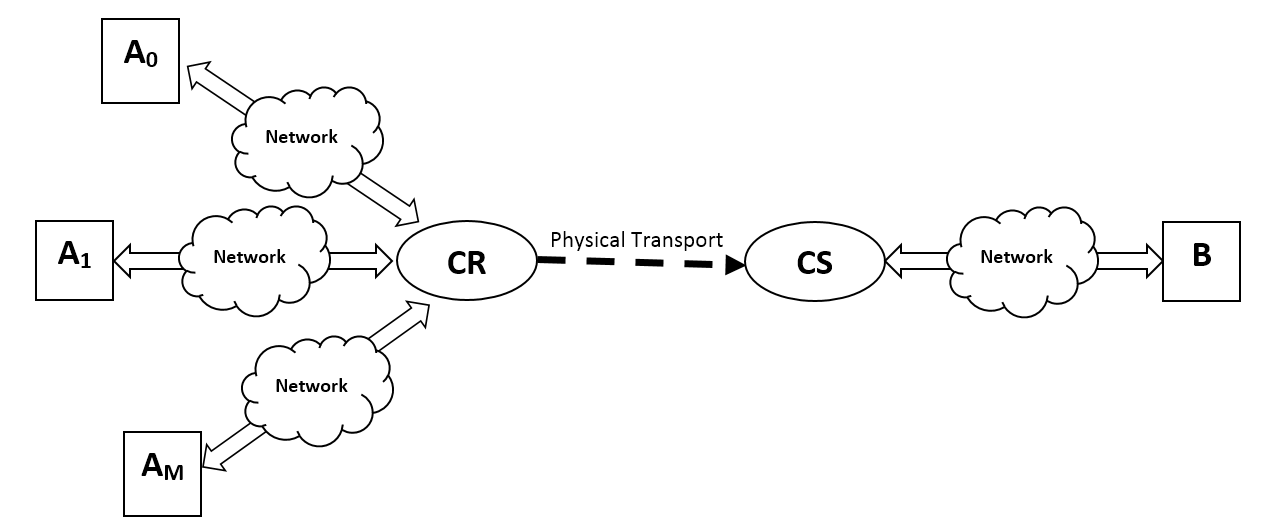
\includegraphics[width=\textwidth,natwidth=1263,natheight=256]{communicationmodel.png}
\caption{Communication Model}
\end{figure}

\subsection*{Adversary Model}

The adversary model in this protocol is mostly derived from Dolev-Yao model which implies ``adversary carries the message" \cite{dolev}. Specifically, adversary $\mathcal{Z}$ has following capabilities:
\begin{itemize}
\item It recognizes the whole system, including communication structure and all information about other members.
\item It can access/rewrite any message passing through the network.
\item It is a legitimate user of the network and it could be any of 4 entities in this protocol.
\item If it is a passive entity (Alice or Bob), it will always have the opportunity to be contacted by any other entities that are capable of (Courier).
\item It can hijack any Courier at any stage of the protocol and get access to all the Courier's data.
\end{itemize}
It should be noted that although the adversary against this protocol has been given great power, its goal is highly restricted - only to reveal the message content sent from Alice to Bob. That means, $\mathcal{Z}$ will not purposelessly hijack a Courier forever or change the data it carries to achieve any other goals (such as DoC attack).

\subsection*{Protocol Properties}
\subsubsection*{Submit protocol}
\begin{itemize}
\item $\mathcal{A}$ is authenticated to $\mathcal{CR}$
\item $\mathcal{A}$ can deny the communication with $\mathcal{CR}$
\item The confidentiality of message content from $\mathcal{A}$ to $\mathcal{B}$ is preserved
\item The Integrity of message from $\mathcal{A}$ to $\mathcal{CR}$ is preserved
\end{itemize}

\subsubsection*{Transmit protocol}
\begin{itemize}
\item $\mathcal{B}$ is authenticated to $\mathcal{CS}$
\item $\mathcal{B}$ can deny the communication with $\mathcal{CS}$
\item The confidentiality of message content from $\mathcal{A}$ to $\mathcal{B}$ is preserved
\item The Integrity of message from $\mathcal{CS}$ to $\mathcal{B}$ is preserved
\end{itemize}

\subsubsection*{On the whole}
\begin{itemize}
\item $\mathcal{A}$ is authenticated to $\mathcal{B}$
\item Non-repudiation for $\mathcal{A}$ to $\mathcal{B}$
\item Confidentiality, integrity of message from $\mathcal{A}$ to $\mathcal{B}$ is preserved
\item Protected from repeat attack
\end{itemize}

\subsubsection*{Properties do not cover}
\begin{itemize}
\item Forward Secrecy and key revocation
\item DoS protection
\end{itemize}

\subsection*{Property Proof}

\begin{thebibliography}{9}
\bibitem{goldwasser}
  Shafi Goldwasser, Silvio Micali, and Ronald Rivest,
  \emph{A digital signature scheme secure against adaptive chosen-message attacks},  SIAM Journal on Computing,
  17(2):281–308,
  Apr. 1988.
  
\bibitem{dolev}
  D. Dolev, A. C. Yao,
  \emph{On the security of public key protocols},
  IEEE trans. on Information Theory,
  IT-29: 198–208,
  1983.
\end{thebibliography}

\end{document}